\section{Assignment 3}

\subsection{Introduction}
\todo{Introduction to the assignment}

\subsection{Autonomous system}
Figure \ref{fig:cell_biology_ex1} shows the continuation of the system with the following parameters (default): $R_0 = 0.3$, $\rho_0 = 0.16$, $\delta R = 1$, $n = 4$, $B_{max} = 0.04$ and $\epsilon = 0.0$. 

\begin{figure}[H]
    \centering
    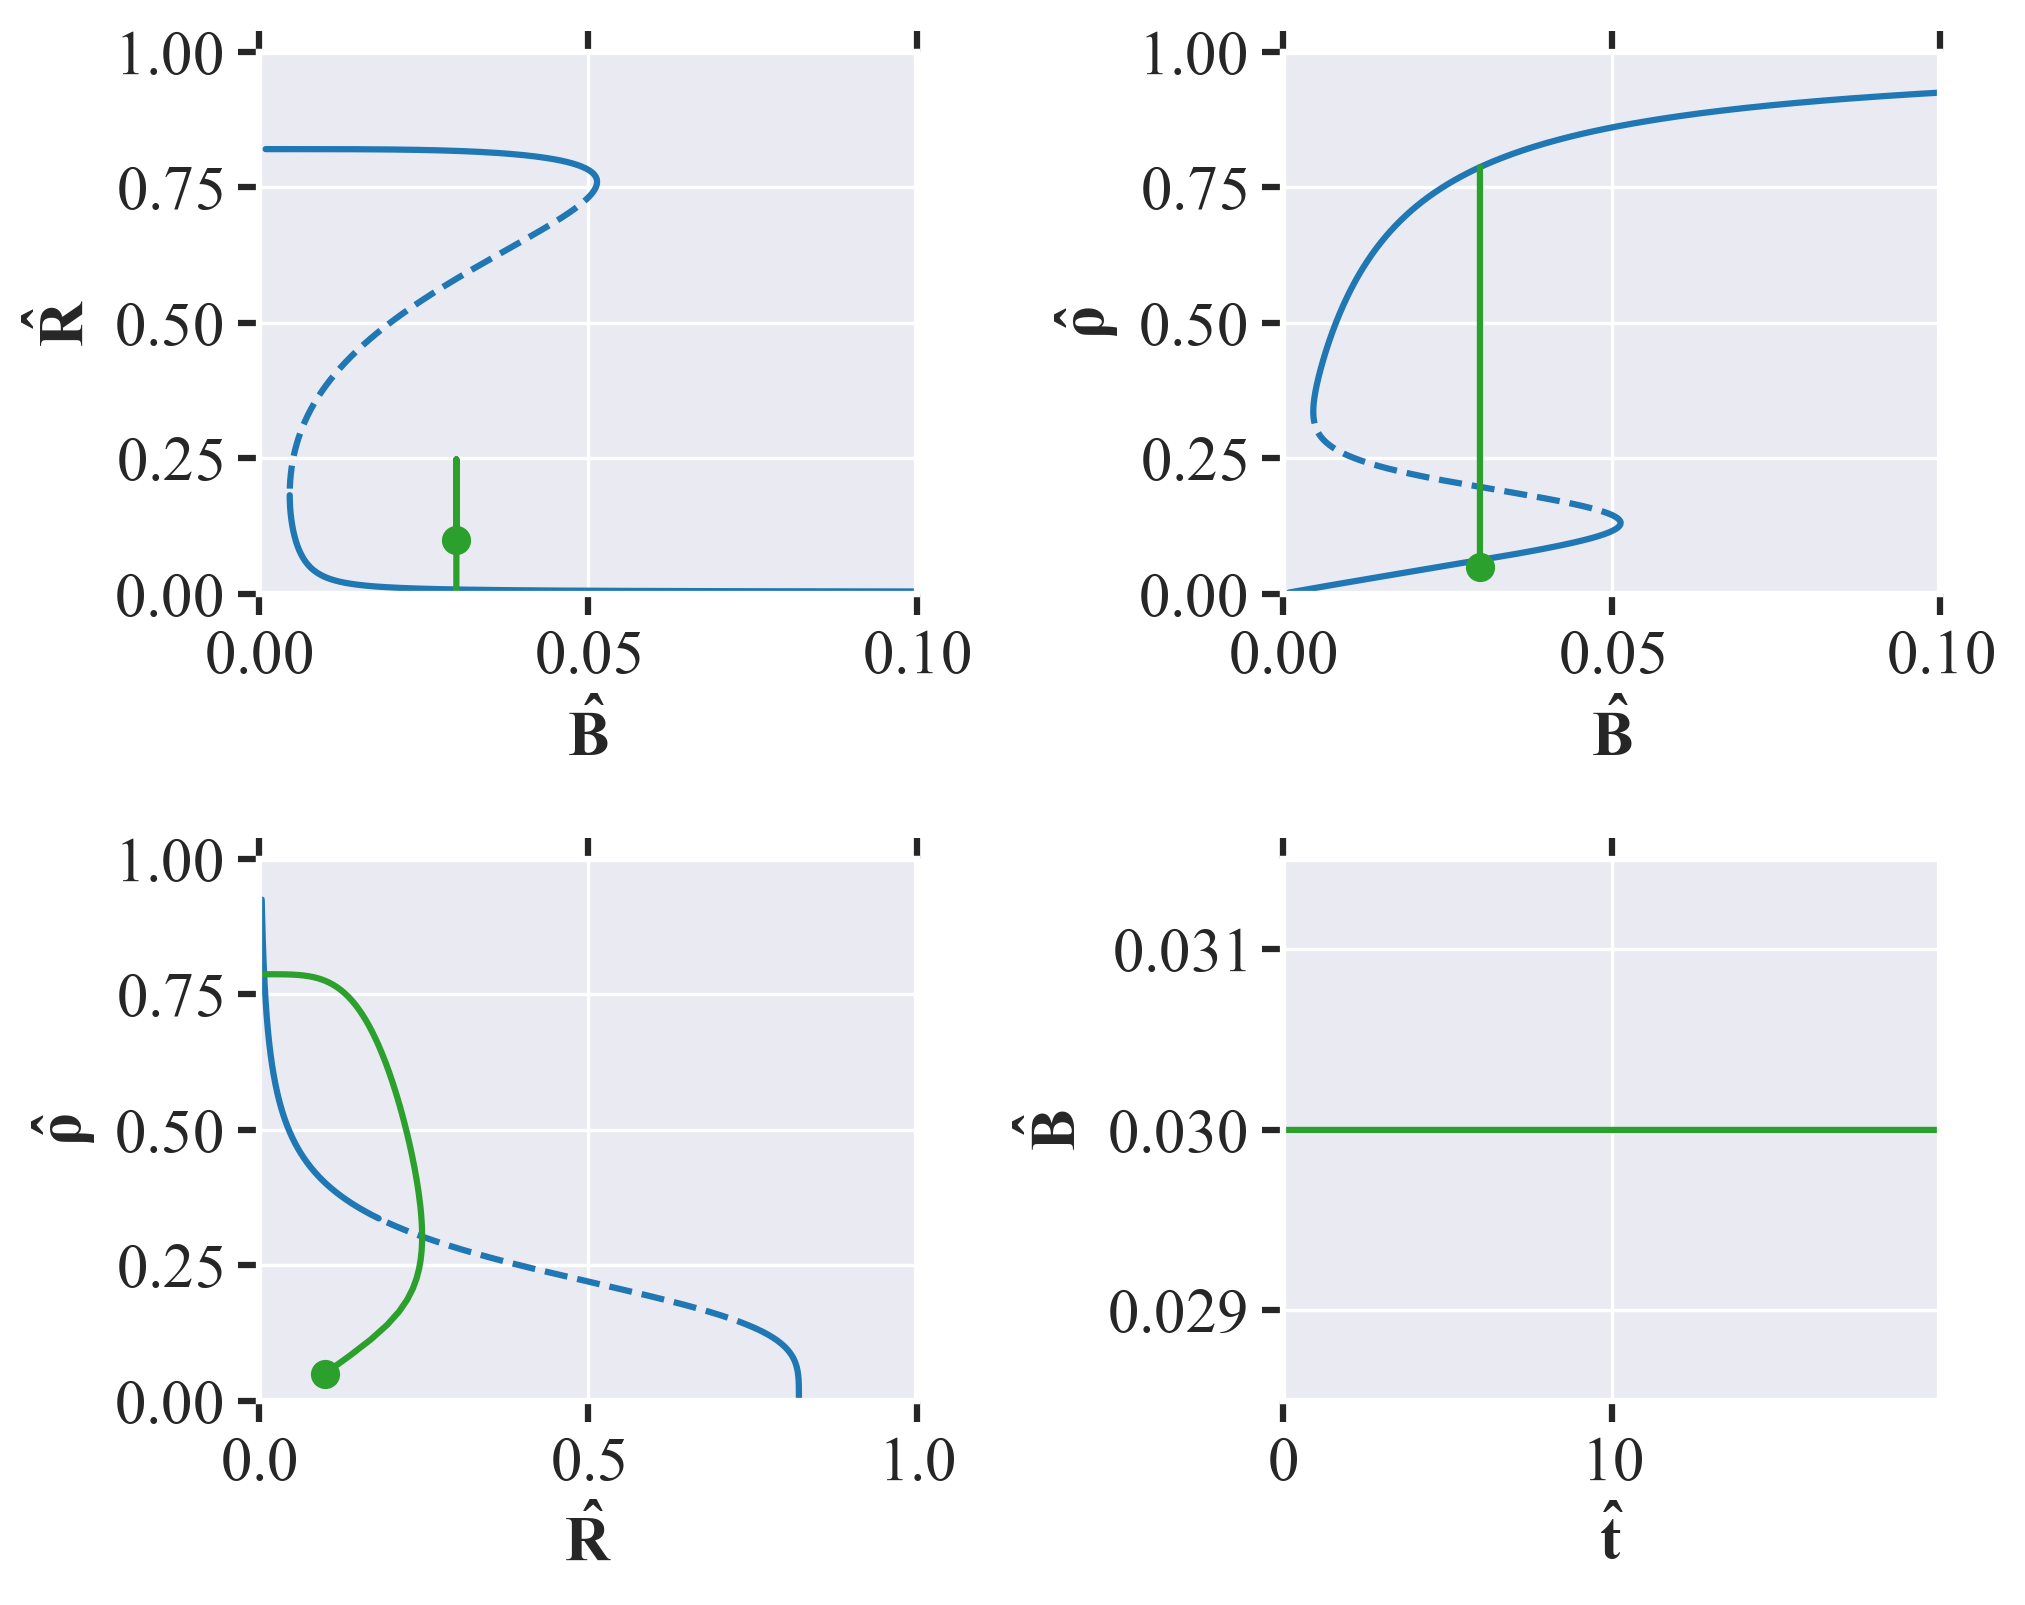
\includegraphics[width= \textwidth]{figures/cell_biology_R0=0.3_rho0=0.16_deltaR=1_n=4_Bmax=0.04_eps=0.0.png}
    \caption{Figure of the continuation of \textbf{top left:} $(\hat{R}, \hat{B})$ and \textbf{top right:}, $(\hat{\rho}, \hat{B})$, \textbf{bottom left:} phase space $(\hat{\rho}, \hat{R})$ and 
    \textbf{bottom right:} $\hat{B}$ against time (time horizon of 20 seconds with a timestep of 0.01). Dots (orange) indicate turning points.}
    \label{fig:cell_biology_ex1}
\end{figure}

The system is at this stage effectively autonomous, since $\hat{B}(\hat{t}) \equiv \hat{B}_c$ is taken to be constant. Continuation is subequently done with respect to the parameter $\hat{B}$. We observe two turning point bifurcations at:
\begin{enumerate}
    \item $\hat{B} \approx 0.051, \hat{R}\approx0.759, \hat{\rho}\approx0.131$; 
    \item $\hat{B} \approx 0.005, \hat{R}\approx0.182, \hat{\rho}\approx0.337$.
\end{enumerate}

Using the graph to get initial guesses for our Newton root finding method, we find there exist three equilibria:
\begin{align*}
    E_0=(\hat{R_a}, \hat{\rho_a}) \approx (0.58,0.20) \leftarrow ||E_0|| \approx 0.61, \\
    E_1=(\hat{R_a}, \hat{\rho_a}) \approx (0.01,0.79) \leftarrow ||E_1|| \approx 0.79, \\
    E_2=(\hat{R_a}, \hat{\rho_a}) \approx (0.82,0.06) \leftarrow ||E_2|| \approx 0.82.
\end{align*}
$E_0$ is unstable, while $E_1$ and $E_2$ are stable. Moroever, looking at the trajectory in the phase space $(\hat{\rho}, \hat{R})$, we see that the system converges to $E_1$. 
Therefore, $E_1$ is the attractor in this case.

In figure \ref{fig:cell_biology_domains_of_attraction} the domains of attraction of $E_i, \ i = 1,2,3$ are shown.
\begin{figure}[H]
    \centering
    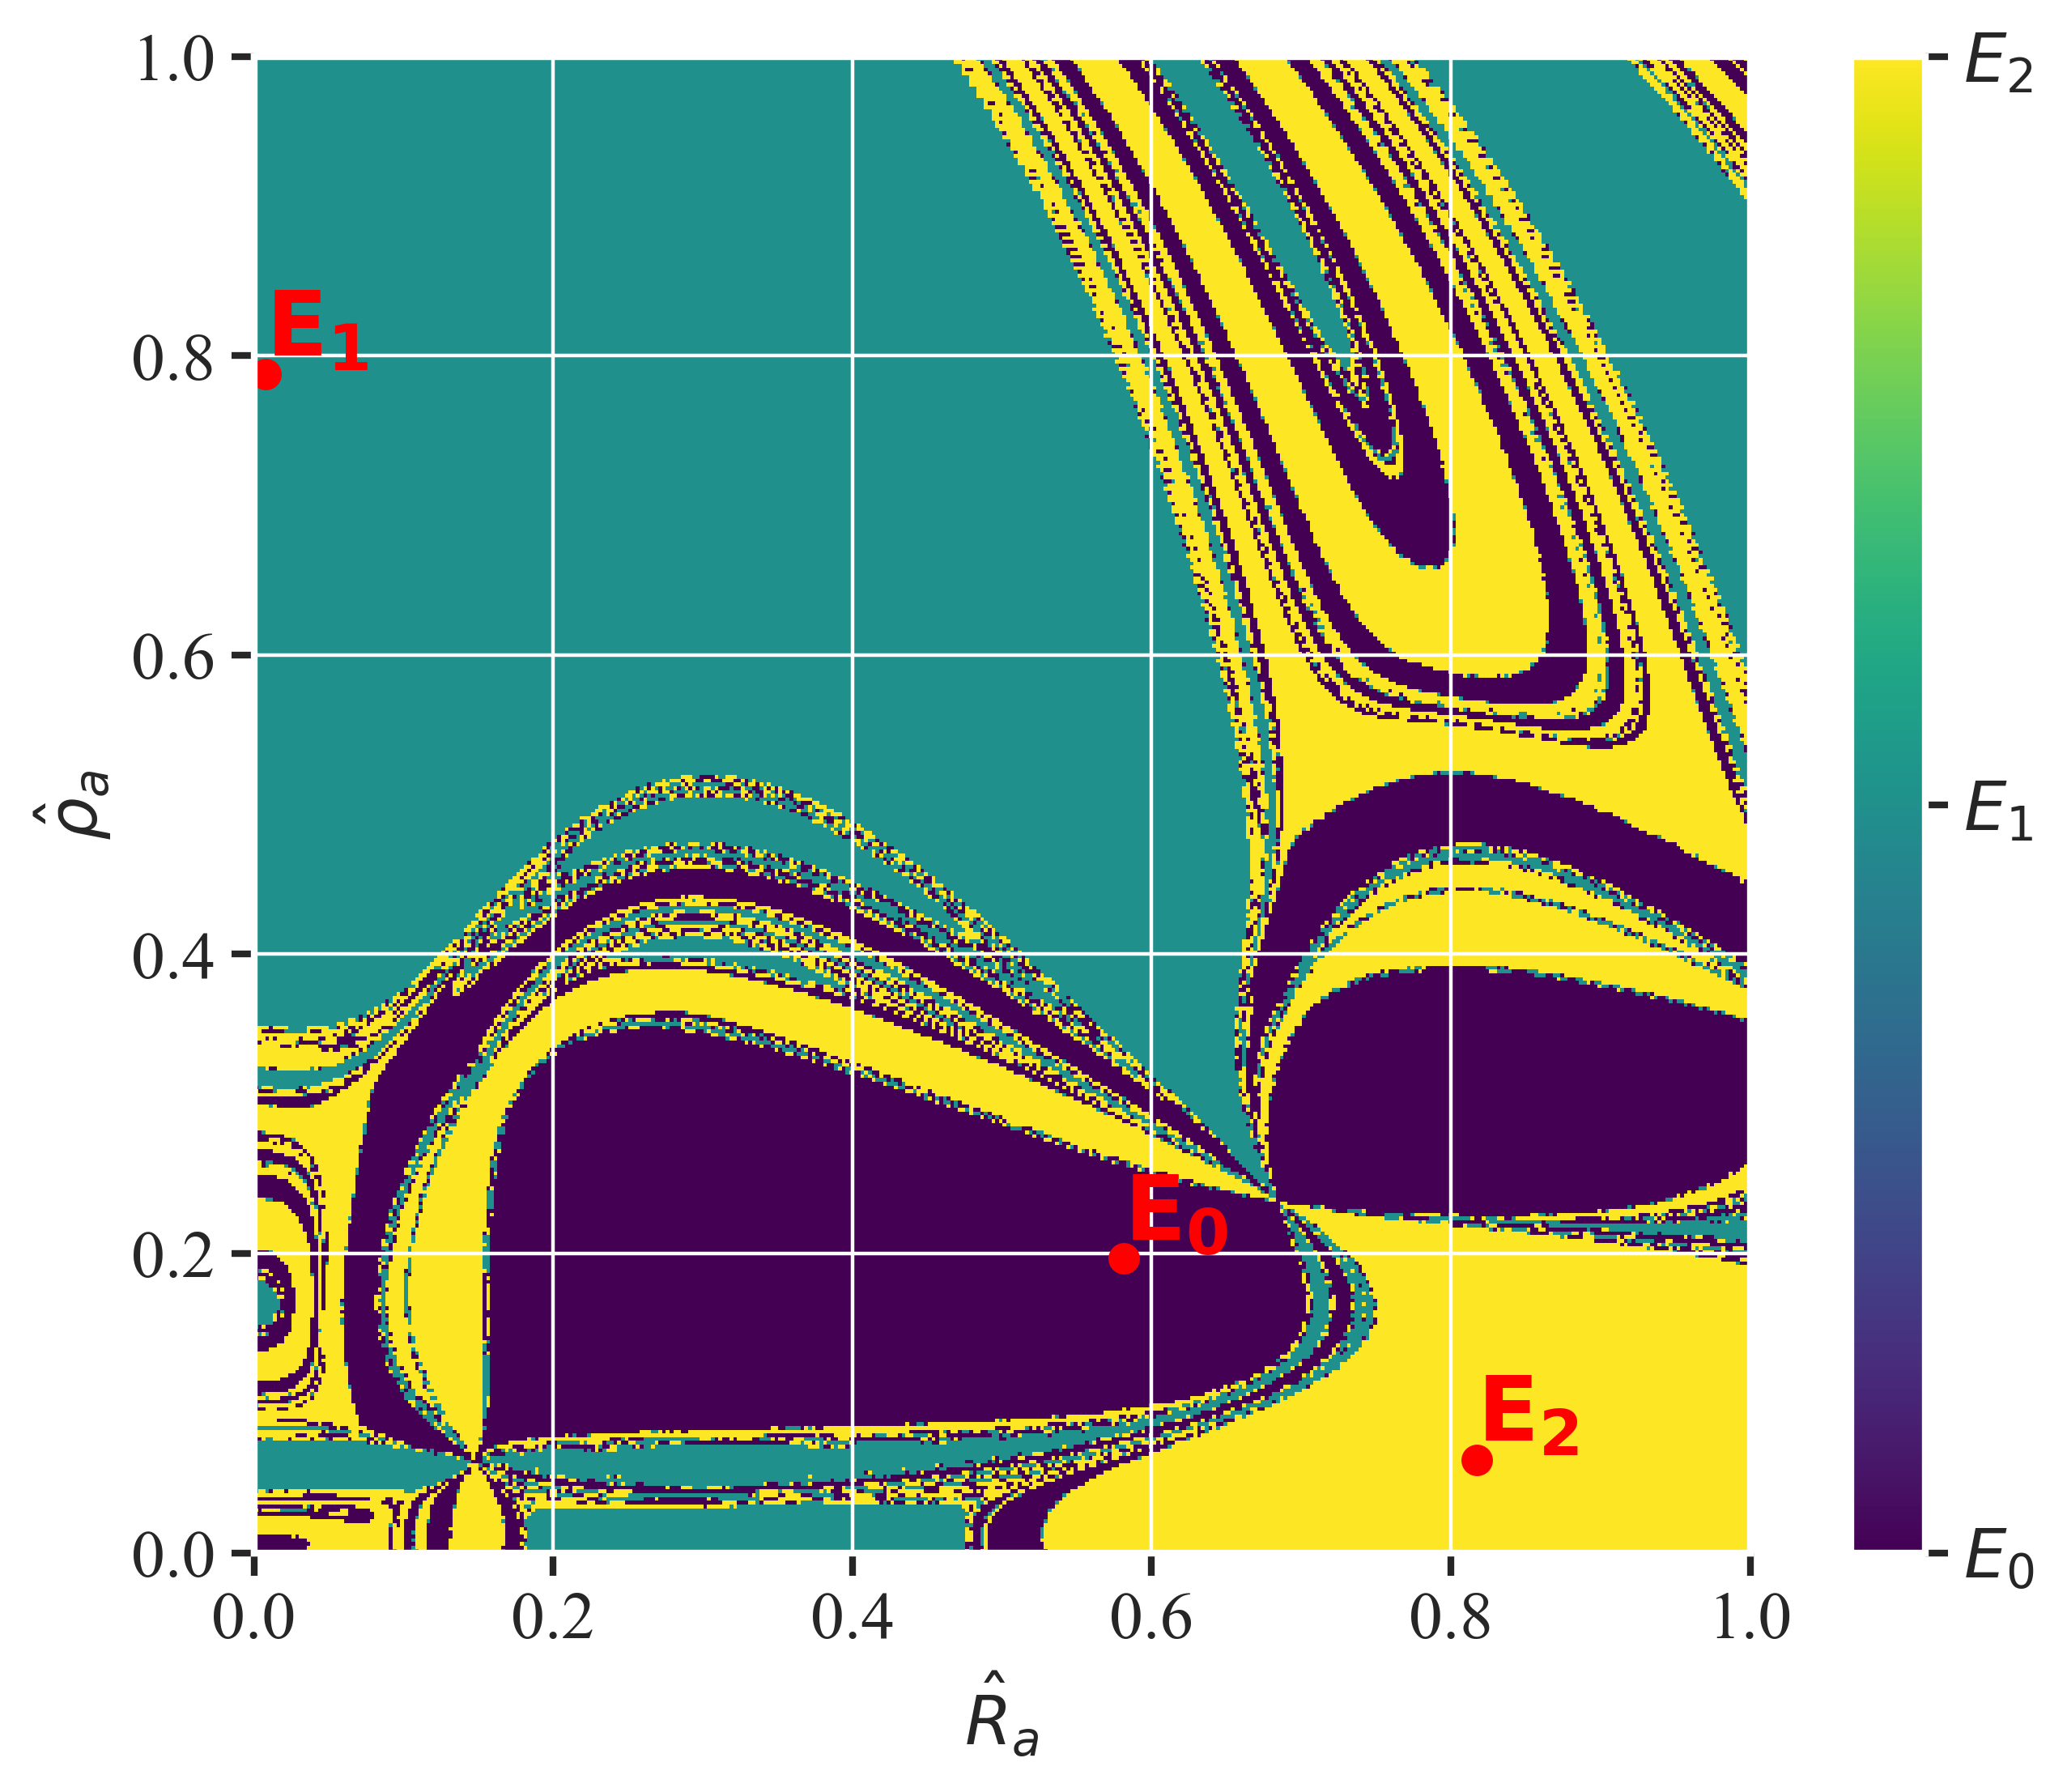
\includegraphics[width= \textwidth]{figures/cb_domains_of_attraction.png}
    \caption{domains of attraction of $E_i, \ i = 1,2,3$}
    \label{fig:cell_biology_domains_of_attraction}
\end{figure}

\subsection{Conclusion}
\todo{Conclusion to the assignment}